\documentclass[twocolumn,11pt]{article}

\usepackage[utf8]{inputenc}
\usepackage{lipsum}                     % Dummytext
\usepackage{hyperref}
\usepackage{xargs}                      % Use more than one optional parameter in a new commands
\usepackage[pdftex,dvipsnames]{xcolor}  % Coloured text etc.
\usepackage{graphicx}
\usepackage{verbatim}
\usepackage{float}
\usepackage{tikz-qtree}
\usepackage{tikz}
\usepackage[linguistics]{forest}

\usepackage{amssymb}
\usepackage{amsmath}
\newcommand*{\QEDA}{\hfill\ensuremath{\blacksquare}}% filled box
\newcommand*{\QEDB}{\hfill\ensuremath{\square}}% unfilled box

% dem nice tables
\usepackage[hmargin=2cm,top=4cm,headheight=65pt,footskip=65pt]{geometry}
\usepackage{fmtcount} % for \ordinalnum
\usepackage{array,multirow}
\usepackage{tabularx}
\usepackage{lastpage}


% add a special collumn type
\newcolumntype{C}[1]{>{\centering\arraybackslash}m{#1}}


%header/footer stuff
\usepackage{fancyhdr}
\pagestyle{fancy}

%note that if you do not do these blank ones, the package defaults to something
%you may not want in your header or footer
\lhead{CMPS 278}
\chead{RocksBench}
\rhead{\today}
\lfoot{Isaak Cherdak}
\cfoot{}
\rfoot{\thepage}

\renewcommand{\headrulewidth}{0pt}
\renewcommand{\footrulewidth}{0pt}

\hypersetup{
    colorlinks=true,
    linkcolor=blue,
    filecolor=magenta,
    urlcolor=cyan,
}

\usepackage[english]{babel}
\emergencystretch=1pt
\usepackage[justification=centering]{caption}
\graphicspath{{Pictures/} }

\usepackage[colorinlistoftodos,prependcaption,textsize=tiny]{todonotes}
\newcommandx{\unsure}[2][1=]{\todo[linecolor=red,backgroundcolor=red!25,bordercolor=red,#1]{#2}}
\newcommandx{\change}[2][1=]{\todo[linecolor=blue,backgroundcolor=blue!25,bordercolor=blue,#1]{#2}}
\newcommandx{\info}[2][1=]{\todo[linecolor=OliveGreen,backgroundcolor=OliveGreen!25,bordercolor=OliveGreen,#1]{#2}}
\newcommandx{\improvement}[2][1=]{\todo[linecolor=Plum,backgroundcolor=Plum!25,bordercolor=Plum,#1]{#2}}
\newcommandx{\thiswillnotshow}[2][1=]{\todo[disable,#1]{#2}}

%\usepackage{setspace}
%\doublespacing

\title{RocksBench\\CMPS 278}
\author{Isaak Cherdak}
%\date{} %blank date

\begin{document}

\maketitle

\pagebreak

\section*{Notation}

\begin{center}
  \begin{tabular}{ | l | l | }
    \hline
    Abbreviation & Expanded Phrase or meaning\\ \hline \hline
    DBMS & Database Management System\\ \hline
    SLA & Service Level Agreement\\ \hline
    WBL & Write Behind Logging \\ \hline
  \end{tabular}
\end{center}

\section{Introduction}
\label{sec:overview}

RocksDB\cite{rocksdb} is a popular DBMS used in applications ranging from
storing data for Netflix to being a component of other database services like
MongoDB. This is very impressive as RocksDB was only designed specifically for
Facebook's needs: to lessen the bottleneck of storage space. The general
philosophy behind RocksDB is that as long as the SLA is met, all optimizations
should be focused on decreasing storage space. However, since the best DBMS
depends on the use case\cite{278:lecture}, it is not completely clear as to what
range of situations would best make use of RocksDB. I present RocksBench, a
simple benchmark that aims to give better insight into the applications where
RocksDB would be especially effective.

RocksBench uses various combinations of calls to RocksDB functions to try to
simulate realistic specialized scenarios. In addition, it allows the user to
tune parameters for testing in as large or small scale as needed. RocksBench
is also able to provide an easy way to visualize results. To this end, there are
a number of scripts provided to analyze the results as well as plot graphs. The
analysis is done using ascar-pilot\cite{li:pilot}. Finally, graphs are generated
via python's matplotlib library.

\section{Background}
\label{sec:background}

\subsection{My Personal Experience}
\label{subsec:personal_experience}

I have experience setting up Benchmarks in C/C++ for various APIs ranging from
custom ones provided by my own data structures to verilog systems.
As an example, in the former system I have been able to send multiple experiment
trials to a file and have used pilot to generate analytics for the results (such
as standard deviation, average, etc). I have also been able to graph these
results using matplotlib. I applied this experience to design an even more
dynamic process of running experiments for RocksDB.

I previously did experiments on four different data structures: Singly Linked
List, Vector, B-Tree, and LSM-Tree. The first three were written by myself in a
consistent manner and the LSM-Tree was adapted based off one created by a
Harvard PhD student. The benchmark was at best able to run 40000 inserts and
40000 get calls with 100 trials in approximately 30 seconds. The order of
inserts and get calls wasn't the same but the way they were run differed
depending on the data structure. The hardware setup was the home PC as described
in \ref{subsec:test_hw} as well as my laptop whose hardware wasn't as powerful
and hence resulted in mostly slower results. Test results included aggregate
runtime of all inserts, aggregate runtime of all calls to get, and total
in-memory size at the end of all insertions. It should be noted that I was able
to run these experiments without having any issues with memory / storage usage
(runtime was main bottleneck) when using an 800 MB NVRAM pool. Valgrind reported
approximately 25 GB of dynamic memory allocating/freeing over the course of all
trials/experiments in the case of 40000 inserts/100 trials.

\subsection{Ascar-Pilot}

Pilot\cite{li:pilot} is an analysis tool created by Yan Li in coordination with
the SSRC. There are three forms: a command line tool for analyzing spreadsheets,
a command line tool for timing a shell command, and a library which can be used
in C++ to time functions. I went with the first system since I was perfectly
fine generating timing data on my own but I have past experience with the third
as well: it just tends to take very long. Pilot was hence used to provide
averages over multiple trials for each type of test as well as variance which
was used to generate error bars for graphs.

\subsection{LSM Trees}

RocksDB is structured based off LSM Trees as was LevelDB\cite{leveldb}. However,
RocksDB makes more interesting use of LSM trees as is described in
\ref{subsec:rocksdb}. Over the course of the development and deployment of
RocksDB, Facebook determined that the most useful properties of the LSM tree
were decreased write and space amplification. Before this discovery, LSM trees
were less popular and their most major benefit was thought to be decreased
random writes to storage.

\subsection{RocksDB}
\label{subsec:rocksdb}

RocksDB\cite{rocksdb} started as a fork of Google's LevelDB\cite{leveldb} and
has made major improvements as well as gained major popularity. Some of the most
notable features which make more interesting use of LSM trees are different
multipliers for the size of a tree component at a given level and unique
treatment to different levels of the tree. For example, in general RocksDB seems
to use the 10x multiplier which provides the interesting property of having the
lowest level of the tree contain 90\% of the data. To help with this, they apply
the strongest compression method to this level of the tree, but no compression
to the highest levels of the tree, and mixed levels in between.

The RocksDB paper gave a lot of insight into the features the system implemented
and how it worked in practice, even though it didn't provide many particularly
novel ideas. A major concern I had with the RocksDB paper was the evaluation
section. It's difficult to fairly compare RocksDB with another system since
RocksDB only intends to meet SLA: any differences in performance between other
systems are kind of irrelevant in this regard. The only metric that mattered was
storage size which wasn't any better than InnoDB (with zlib compression) and
TokuDB (with no compression). As such, the message appears to be that RocksDB
maintains only reasonable storage optimization while also giving reasonable
performance. However, that isn't to say that RocksDB can't be used as a database
for its performance characteristics.

\section{Motivation}

The motivation behind this project was to try to observe some special use cases
of RocksDB and make interesting conclusion about them. In addition, the
motivation was to fulfill the requirements of my class project. Initially the
project had the following levels of expectation, where I would say that I have
very substantially completed level A.

\subsection{Level A}

Characterization of major use cases of RocksDB and discussion of optimizations
that would further increase the range of use cases. This involves running
various benchmarks and analysis of the results as described in
\ref{subsec:characterization_tests}.

\subsection{Level B}

This involves the work proposed in Level A as well as tests on an optimized
version of RocksDB. This optimization would likely be a modified version of
RocksDB so that it runs on NVRAM as described in \ref{subsec:nvram}.

\subsection{Level C}

This would involve Level A, B, and the application of Levels A and B to LevelDB.
Finally, a comparison of the use cases between the two systems which will simply
include the Level A analysis of both systems. This would also include a
discussion of the cost-benefit of some of the features added to RocksDB which
LevelDB did not have.

\section{RocksBench}

\subsection{Overview}

This Benchmark was designed in C++ and provides command line arguments to let
users customize options for the tests. The Benchmark provides the user the
ability to customize operation and automates the process of visualizing results.

\subsection{Characterization of tests}
\label{subsec:characterization_tests}

\begin{table}[h!]
  \begin{tabular}{ |c|c|c|c| }
    \hline
    Test Name & R:W:D Ratio & Hit Rate & Data \\
    \hline \hline
    seq\_hit\_read & 1000:10:5 & High & Seq \\ \hline
    seq\_hit\_write & 10:1000:5 & High & Seq \\ \hline
    seq\_hit\_delete & 100:10:50 & High & Seq \\ \hline
    seq\_miss\_read & 1000:10:5 & Low & Seq \\ \hline
    seq\_miss\_write & 10:1000:5 & Low & Seq \\ \hline
    seq\_miss\_delete & 100:10:50 & Low & Seq \\ \hline
    rnd\_hit\_read & 1000:10:5 & High & Rnd \\ \hline
    rnd\_hit\_write & 10:1000:5 & High & Rnd \\ \hline
    rnd\_hit\_delete & 100:10:50 & High & Rnd \\ \hline
    rnd\_miss\_read & 1000:10:5 & Low & Rnd \\ \hline
    rnd\_miss\_write & 10:1000:5 & Low & Rnd \\ \hline
    rnd\_miss\_delete & 100:10:50 & Low & Rnd \\ \hline
  \end{tabular}
  \caption{The twelve different types of tests}
  \label{tab:types_of_tests}
\end{table}

There are twelve different kinds of tests as described in table
\ref{tab:types_of_tests}. Each test strives to show the results of using a
different kind of input set. Basically, the three parameters which are cycled
include: the type of operation to emphasize, the hit rate, and whether the data
is random or sequential. The individual R:W:D values in the above ratio are done
\$size times: this way you can use a variety of different input sizes but still
maintain the ratio as described above.

\subsection{Implementation}
\label{subsec:implementation}

RocksBench was designed very carefully in the interest of modularity as well as
to prevent unnecessary operations. This is important as the RocksDB library
functions already take up a large portion of the benchmark runtime. It is also
relatively scalable: being able to perform tests with very large base sizes as
illustrated in \ref{subsec:max_threshold}.

\subsubsection{Main System}

This facilitates handling all the command line arguments and calling each
benchmark test as needed. Once command line arguments are parsed and handled,
the system begins to call all twelve tests for every size in the set requested.
In addition, it runs multiple trials on each test as specified by the user. The
results vector is taken from the returning trials and appended to a csv named
based on the test type and size of test. In addition, it ensures that the first
line is a header which can be constructed after the first trial.

\subsubsection{Benchmark}

This contains the code for all the benchmarks. Operations are always in the
order: write, read, delete. This is because writes need to occur before anything
else, reads are only interesting if the database is already at the specified
size, and deletes must thus be last. These benchmarks are very similar: only
containing very small nuances depending on the parameter. To ensure ratios, a
given operation is done size*ratio times. For example, on size 100, test
seq\_hit\_write would perform 100000 writes, 1000 reads, and 500 deletes.
Furthermore, high hit rate would make reads always read data that was already
inserted whereas low hit rate would make reads attempt to poll for data that
isn't there or in the case of random, likely isn't there. Finally, Sequential
data is generated via a loop from some starting value to guarantee some provided
average while random data is a Poisson distribution around the provided average
value. I tried to keep the average value the same between sequential and random
data since I wasn't varying spatial locality and hence wanted to keep it
controlled. The output of a benchmark is a vector of tuples containing
(name\_of\_value, value). Currently there are only three: total put() time,
total get() time, and total delete() time. Note that the total includes only
size operations. To accomplish this, I simply divide the total time result by
the relative ratio of an operation for a given test. Finally, all of these
results are returned in milliseconds to be placed on a csv by the Main System.

\subsubsection{RocksUtil}

This is a wrapper around the library functions of RocksDB. It provides
functionality for creating and destroying a database, the basic put(), get, and
delete calls, as well as the use of committable transactions for put() and
get(). The transactions functions were not used in this project.

\subsubsection{analysis scripts}

There are two analysis scripts. analyze\_results.sh runs pilot on all three
fields of the results and makes a .txt file for the results of the put(), get(),
and delete() columns. analyze\_all.sh performs analyze\_results.sh on all of the
csv files in all results folders and respective subfolders. In addition, it
creates an analysis folder and fills it with a comprehensive
(size,mean,variance) compilation of all pilot results for all size for a given
type of test.

\subsubsection{Plotting scripts}

plot\_results.py is a python program which is designed to take the compiled
final results from analyze\_all.sh and turn them into graphs. Similarly to
analyze\_all.sh, plot\_all.sh simply runs plot\_results.py on every
comprehensive analysis file in all of the subfolders of all results folders.

\subsection{usage}

\begin{table}[h!]
  \begin{tabular}{ |c|c|c|c| }
    \hline
    Option & Description & input type \\
    \hline \hline
    n & specify prefix for results folder & string \\ \hline
    b & beginning size & int \\ \hline
    s & end size & int \\ \hline
    m & amount to increase (multiply) size & float \\ \hline
    t & number of trials & int \\ \hline
    d & debug & None \\ \hline
  \end{tabular}
  \caption{A list of all the options available in RocksBench}
  \label{tab:RocksBench_options}
\end{table}

The Main system allows a user to choose some options. These are listed in table
\ref{tab:RocksBench_options}. Together with these options you can perform tests
according to your needs. RocksBench will run all twelve of the tests described
in section \ref{subsec:characterization_tests} for all sizes starting at the
beginning value, multiplying by the multiplier each time, and going until the
value is bigger than the end size. The folder will be <custom\_name>\_results
where <custom\_name> is "default" by default and configured with the -n option.

The flow of getting results is very simple with RocksBench. Files are organized
in a hierarchy of custom\_result/test\_type/test\_type\_size.csv. Once RocksDB
is run to generate these files, one can use run.sh which calls the other four
scripts as needed to generate graphs and copy them to
figures/<results\_prefix>/<test\_type>\_complete\_<op\_name>.png.

\section{Evaluation}

A lot of graphs were generated due to the ease of use of RocksBench.
Specifically, there were 72 graphs at the end of my experiments. This is because
there is a graph for every operation (put, get, delete) for every type of test
(for which there are 12) and for both computers (my home and lab computer).
Thus, not all graphs are displayed here but they can be viewed here:
\href{https://github.com/legendddhgf/Database_Systems_Project/tree/master/project/doc/Pictures}
{RocksBench Graphs}.
In addition, error bars are implemented but apparently 10 trials was sufficient
to make matplotlib not even display the error bars for most data points.

\subsection{Test Hardware}
\label{subsec:test_hw}

I ran these tests on a virtual machine on my home desktop as well as on a direct
boot of Linux on my lab machine. My home desktop has an AMD Ryzen R7 1700 CPU,
32 GB 3000MHz DDR4 RAM, and a 500 GB primary storage SSD. The virtual machine
uses 8 CPU cores, 16 GB RAM, and 50 GB of my SSD. As for my lab PC, it has an
Intel core i5-3550 CPU, 16 GB 1866MHz DDR3 RAM, a 500 GB SSD, ~250 GB of which
are being used for the Linux installation.

\subsection{Maximum Threshold}
\label{subsec:max_threshold}

The range of tests were as large as possible. Experiments were run from 1 to
32768 base size, taking somewhere around 4 hours to finish on both computers.
The next size up, 65536, would actually be stuck on the first trial of
seq\_miss\_read which makes sense because this test was an anomaly for reasons
such as overturning the general rule of put() being the fastest operation as
one would expect in an LSM Tree based system.

\subsection{Home PC}

\begin{figure}[h!]
  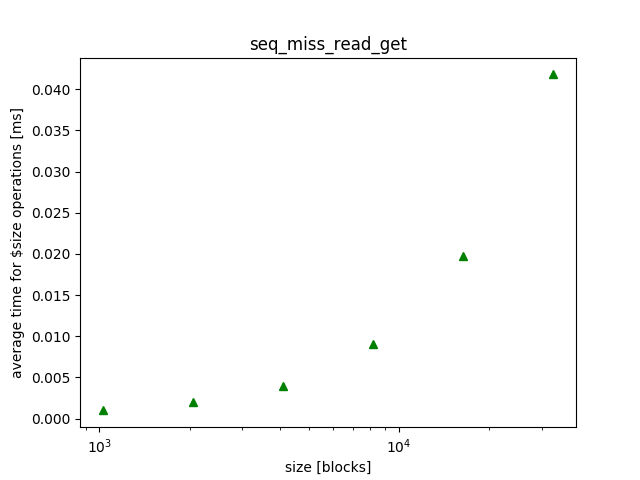
\includegraphics[width=\linewidth]{Pictures/HOMEPC/seq_miss_read_complete_get.png}
  \caption{home\_seq\_miss\_read\_get}
  \label{fig:home_seq_miss_read_get}
\end{figure}
\begin{figure}[h!]
  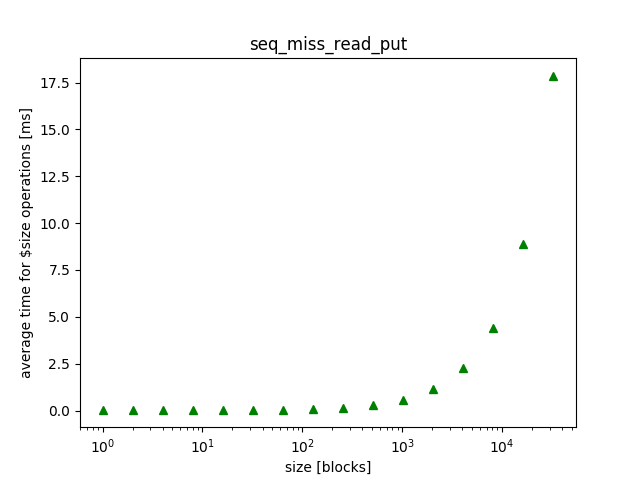
\includegraphics[width=\linewidth]{Pictures/HOMEPC/seq_miss_read_complete_put.png}
  \caption{home\_seq\_miss\_read\_put}
  \label{fig:home_seq_miss_read_put}
\end{figure}
\begin{figure}[h!]
  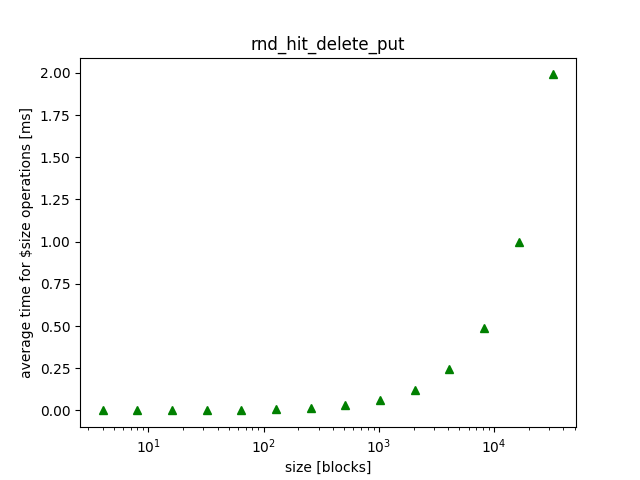
\includegraphics[width=\linewidth]{Pictures/HOMEPC/rnd_hit_delete_complete_put.png}
  \caption{home\_rnd\_hit\_delete\_put}
  \label{fig:home_rnd_hit_delete_put}
\end{figure}
\begin{figure}[h!]
  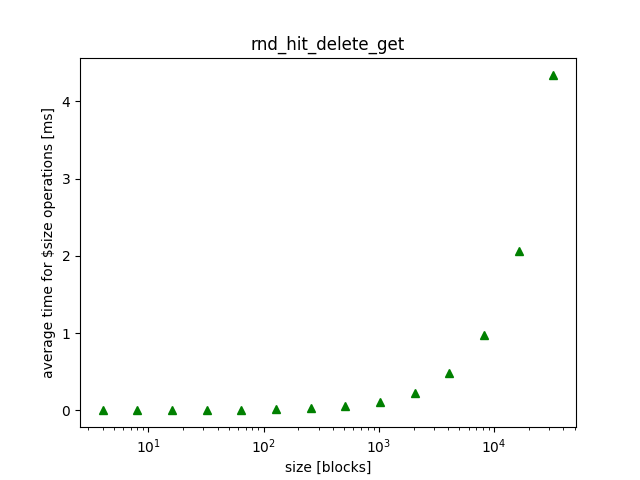
\includegraphics[width=\linewidth]{Pictures/HOMEPC/rnd_hit_delete_complete_get.png}
  \caption{home\_rnd\_hit\_delete\_get}
  \label{fig:home_rnd_hit_delete_get}
\end{figure}
\begin{figure}[h!]
  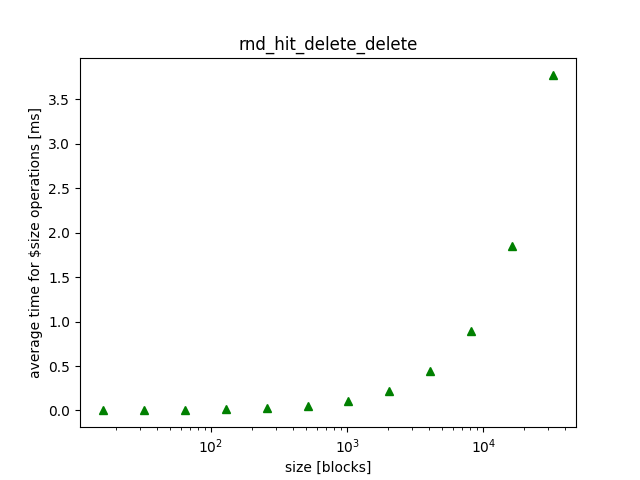
\includegraphics[width=\linewidth]{Pictures/HOMEPC/rnd_hit_delete_complete_delete.png}
  \caption{home\_rnd\_hit\_delete\_delete}
  \label{fig:home_rnd_hit_delete_delete}
\end{figure}

This computer performed much better, likely because of its more modern hardware.
Interestingly enough, it didn't seem to make full use of resources. For any
given test, put() was the fastest except for one case: seq\_miss\_read where
get() was multiple orders of magnitude slower. This can be seen in figures
\ref{fig:home_seq_miss_read_get} and \ref{fig:home_seq_miss_read_put}. Another
interesting group of results is rnd\_hit\_delete in which the time for each
operation is actually pretty similar. These are figures
\ref{fig:home_rnd_hit_delete_put}, \ref{fig:home_rnd_hit_delete_get}, and
\ref{fig:home_rnd_hit_delete_delete}.

\subsection{Lab PC}

\begin{figure}[h!]
  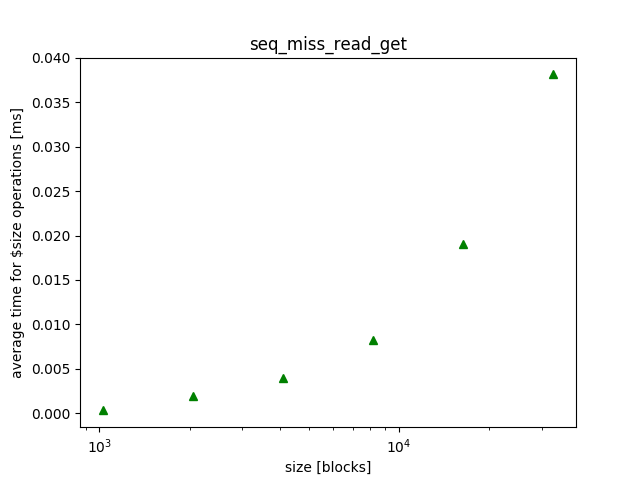
\includegraphics[width=\linewidth]{Pictures/LABPC/seq_miss_read_complete_get.png}
  \caption{lab\_seq\_miss\_read\_get}
  \label{fig:lab_seq_miss_read_get}
\end{figure}
\begin{figure}[h!]
  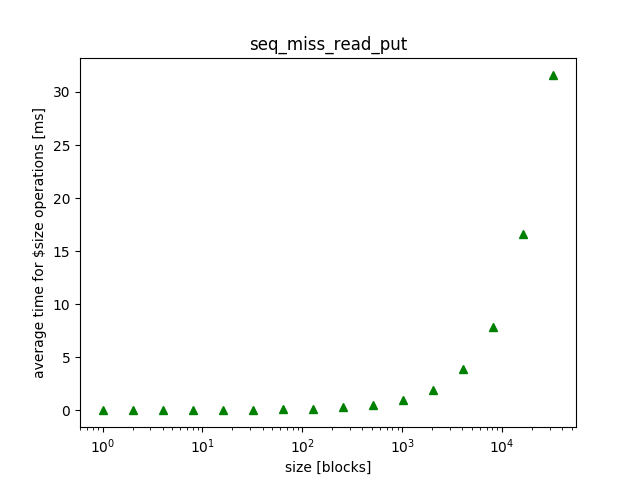
\includegraphics[width=\linewidth]{Pictures/LABPC/seq_miss_read_complete_put.png}
  \caption{lab\_seq\_miss\_read\_put}
  \label{fig:lab_seq_miss_read_put}
\end{figure}
\begin{figure}[h!]
  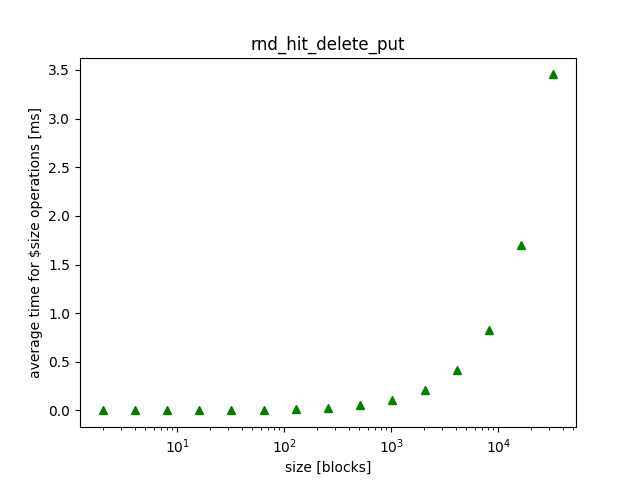
\includegraphics[width=\linewidth]{Pictures/LABPC/rnd_hit_delete_complete_put.png}
  \caption{lab\_rnd\_hit\_delete\_put}
  \label{fig:lab_rnd_hit_delete_put}
\end{figure}
\begin{figure}[h!]
  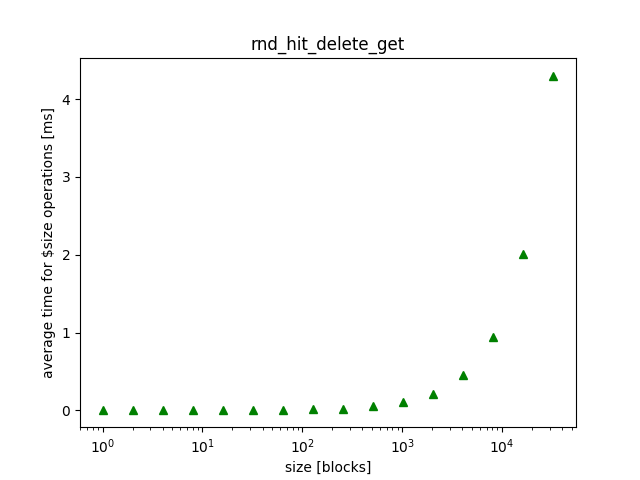
\includegraphics[width=\linewidth]{Pictures/LABPC/rnd_hit_delete_complete_get.png}
  \caption{lab\_rnd\_hit\_delete\_get}
  \label{fig:lab_rnd_hit_delete_get}
\end{figure}
\begin{figure}[h!]
  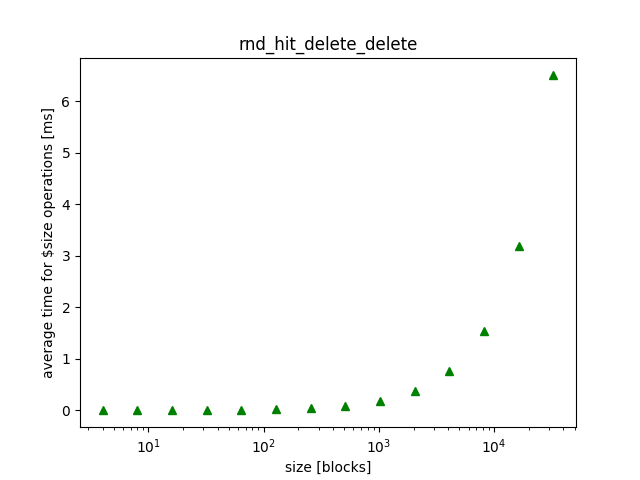
\includegraphics[width=\linewidth]{Pictures/LABPC/rnd_hit_delete_complete_delete.png}
  \caption{lab\_rnd\_hit\_delete\_delete}
  \label{fig:lab_rnd_hit_delete_delete}
\end{figure}

This computer was making heavy use of resources, but even so it was
unsurprisingly slower due to comparatively dated hardware. It had a similar
experience specifically with seq\_miss\_read which can be seen in figures
\ref{fig:lab_seq_miss_read_get} and \ref{fig:lab_seq_miss_read_put}. Similarly
to my home computer, the lab computer observed similar results from all
operations in rnd\_hit\_delete which can be found in figures
\ref{fig:lab_rnd_hit_delete_put}, \ref{fig:lab_rnd_hit_delete_get}, and
\ref{fig:lab_rnd_hit_delete_delete}.

\subsection{Result Insights}
\label{subsec:res_insights}

I observed some interesting results over the course of the variety of tests
performed. Surprisingly, get() is still very fast in many situations: contrary
to what one would expect from a LSM tree. However, delete was perhaps the
biggest hit to latency as it would often take very long for few deletes relative
to the number of reads and writes.

Some work could potentially go into figuring out the most optimal hardware. It
was noted that when running tests on the lab computer, one core was often at
100\% while others were down to around 20-30\% utilization. Perhaps this is an
issue only in older processors but my home computer is actually experiencing the
opposite effect. One might expect my home computer to be much faster than the
lab computer given that the former runs at around 10\% CPU usage. However, even
though it is a little faster, it doesn't seem to be making good use of hardware.
Another factor that may cause this is the virtual machine. However, in the past
I have seen CPU, disk, and memory usage go up to 100\% due to processes in a
virtual machine and currently RocksBench has a negligible affect on both of
these resources.

\subsection{Challenges}

\subsubsection{Benchmark Design}

Designing the benchmark took a large amount of time and consideration because at
any given point the things that I wanted to test could change. If the system was
badly written, there would be a large amount of time spent on rewriting large
portions of the system every time a change occurred.

\subsubsection{Utilization of RocksDB library}

The RocksDB library via the github repo didn't have the best example setup so
some time was spent on coming up with a more generalist configuration.
Originally, RocksDB intended for people to use their examples which were
completely hard-coded to make use of a parent directory as the source for
RocksDB libraries. I remade their examples and Makefiles so that compilation was
based off the actual install directory. This was very good for me because by the
time I wanted to make use of the library, I already knew exactly how to
correctly link it to the install locations and make use of their custom
configuration file. The other major challenge was the sheer number of ways that
you can do a single put/get/delete which is why a lot of the tests I use have
very simple functionality.

\subsubsection{Test Coverage}

Determining the tests to run was very difficult both due to initial concerns and
those that turned up over the course of the project. Initially, I was aware that
there would be a large number of parameters and as a result, it would be
impossible to make a completely comprehensive test. This led me to choose to
leave options as defaults, which may be something that plenty of users would do
for the same reason. I also initially planned to use varying ratios of
\textit{put}, \textit{get}, \textit{update}, and \textit{delete} calls. However,
as the project progressed I realized that the tests that involved random number
generation resulted in \textit{update} calls during what was supposed to be a
\textit{put} test. As a result, I decided to remove \textit{update} tests from
the variables.

\section{Future Work}
\label{sec:future_work}

\subsection{RocksDB using NVRAM}
\label{subsec:nvram}

Many additional optimizations are available to systems that have NVRAM. The most
interesting ones appear to be WBL\cite{Arulraj:2016:WL:3025111.3025116} and the
ability to not always have to flush data from memory to storage. Some
interesting results could be achieved if a variety of ratios of RAM vs NVRAM
were used to benchmark a NVRAM functioning RocksDB.

RocksDB can be modified to use NVRAM with moderate effort. Furthermore, even
with difficulty to attain physical NVRAM, it is possible to emulate it using
Intel's step-by-step guide\footnote{
  \href{https://software.intel.com/en-us/articles/how-to-emulate-persistent-memory-on-an-intel-architecture-server/}
  {Intel NVRAM Emulation Guide}}.
To make use of the NVRAM, regardless of whether it's emulated, the Intel PMDK
library can be used (formerly known as NVML). A perfectly sufficient module
provided by PMDK called libpmemobj
\footnote{\href{http://pmem.io/pmdk/libpmemobj/}
{PMDK libpmemobj documentation}} allows a user to make use of syntax reminiscent
of malloc and free while also providing a persist call.

\subsection{Expanding coverage of the testbench}

RocksBench currently only makes use of very simple calls to RocksDB using the
default options. On one hand this isn't so bad since many users may choose to do
the same since Facebook has chosen default options quite reasonably and because
of the overwhelming variety of methods to make use of the Database. However,
transactions would likely also be used as well as methods common with the
backwards compatible LevelDB API. Luckily, the structure of the database is very
modular and would make such additions relatively painless once they are
independently planned and designed. In addition, perhaps storage size could be
considered, partly as verification that RocksDB is really as space efficient as
claimed.

\subsection{Research into optimal hardware setup}

As mentioned before like in section \ref{subsec:res_insights}, there may be more
nuance than has ever been considered regarding the kinds of hardware that makes
the database system operate more efficiently.

\section{Conclusion and Acknowledgments}

I want to thank Shel for teaching this class and for being such a considerate
advisor during the course. The help I received to determine what my project
should be as well as to plan out the full extent of the project was beyond
anything I have received from any instructor in the past. I would also like to
thank Daniel Bittman for being so active in the class and keeping the knowledge
flowing when no one else had any input. I have returned the favor by adding
error bars to my graphs.

\bibliographystyle{abbrv}
\bibliography{rocksbench,bib/csrg}

\end{document}
